\chapter{Aufbau}

%abbildung von aufbau einfügen
\section{Technische Hintergründe zum Aufbau}
\subsection{Funktionsweise des Szintillationsdetektor}
Ein Szintillationsdetektor (Abbildung \ref{fig:scintillator}) wandelt die Energie ionisierender Strahlung in sichtbares Licht um, das anschließend im Photomultiplier (Abbildung \ref{fig:pmt}) zu elektrischen Signalen verstärkt wird. Ein einfallendes Gammaquant erzeugt im Kristall ein schnelles Elektron, das seine Energie durch Ionisation und Anregung abgibt und dabei Szintillationslicht erzeugt. Die Lichtmenge ist proportional zur deponierten Energie.

Beim NaI(Tl)-Detektor sorgen Thallium-Aktivierungszentren für effiziente Lichtemission. Der Kristall liefert eine hohe Lichtausbeute und eine Abklingzeit von etwa 230 ns. Das Licht gelangt über reflektierende Oberflächen zur Photokathode des PMT, wo es über den photoelektrischen Effekt Elektronen freisetzt. Diese werden in der Dynodenkette vervielfacht und erzeugen einen verstärkten Stromimpuls, dessen Amplitude direkt der deponierten Energie entspricht.


Ein Nachteil von Szintillationsdetektoren ist ihre begrenzte Energieauflösung (für NaI(Tl) ungefär 6\% bei 662keV), bedingt durch statistische Schwankungen der Lichtausbeute und unvollständige Lichtsammlung im PMT. Dafür bieten sie aber eine hohe Effizienz und schnelle Signalantworten, was sie für bestimmte Anwendungen sehr nützlich macht.\cite{Wermes}
\begin{figure}[H]
    \centering

    \begin{subfigure}[t]{0.48\textwidth} %bild szintillationsdetektor
        \centering
        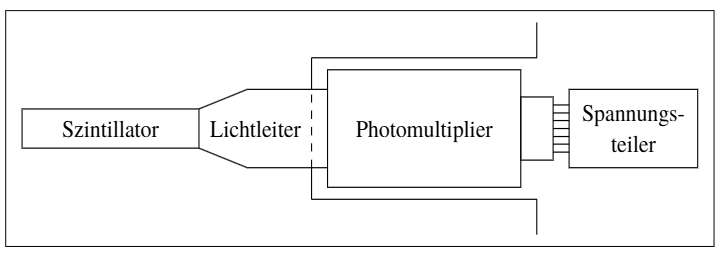
\includegraphics[width=\linewidth]{figs/szintillationszähler.png}
        \caption{Aufbau eines Szintillationsdetektors \cite{praktikum}}
            \label{fig:scintillator}
    \end{subfigure}
    \hfill
    \begin{subfigure}[t]{0.48\textwidth}%bild photokathode
        \centering
        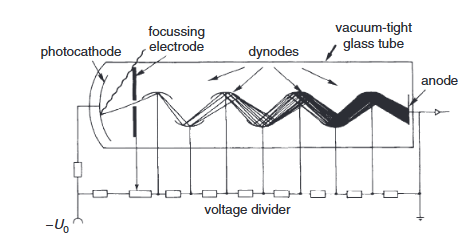
\includegraphics[width=\linewidth]{figs/pmt_image.png}
        \caption{Aufbau eines Photomultipliers \cite{Grupen_2}. Das Elektrodensystem ist in einer evakuierten Glasröhre montiert. Der Photomultiplier wird üblicherweise durch einen Mu-Metall-Zylinder aus hochpermeablem Material gegen magnetische Streufelder abgeschirmt.}
            \label{fig:pmt}
    \end{subfigure}
\end{figure}
Ein Diskriminator erzeugt aus einem Eingangsimpuls mit variabler Amplitude ein amplitudenunabhängiges Zeitsignal. Dieser gibt ein Signal aus, sobald der gemessene Wert der Spannung eine eingestellte Schwellenspannung $U_\text{threshold}$ überschritten hat. Ziel ist es, diese Spannung so einzustellen, dass der Diskriminator die Messung nur dann aufnimmt, wenn der einkommende Impuls von einem Muon kommt, und nicht von elektronischen oder thermischen Rauschen.
Dafür wird die Schwellenkurve der Spannung bestimmt. Indem man das Extremum der Schwellenkurve bestimmt, kann man für einen gewählten energetischen Bereich die passende Schwellenspannung bestimmen.
\subsection{Koinzidenzmessung}
Eine Koinzidenz wird als wahre Koinzidenz bezeichnet wenn ein physikalischer Prozess Ursache von beiden Signalen ist, dass heißt, wenn sie während den Prozess zeitgleich ankommen/ zeitlich korreliert sind.
Hingegen werden Koinzidenzen bei welchen beide Signal unabhängig voneinander sind als zufällige Koinzidenzen betrachtet. Die zufälligen Koinzidenzen werden von den gesammten gemessenen Koinzidenzen abgezogen, da man nur wahre Koinzindenzen für die Auswertung der Messdaten betrachtet.
Dafür werden bei den Detektoren zur gleichen Zeit zwei Messungen von den zufälligen Koinzidenzen durchgeführt. 
\subsection{FPGAs}
Ein Field Programmable Gate Array besteht aus einer integrierten Schaltung, die aus einer Gruppe programmierbarer Logikblöcke besteht. Diese sind durch programmierbare Verbindungen miteinander verknüpft. 
\subsection{LabView}
Im Laufe des Versuchs wir das Programm LabVIEW zur Aufnahme von Messdaten verwendet. Dieses Programm übernimmt die vollständige Steuerung und Auslesung der NIMBox und initialisiert die Treiberbibliothek, öffnet die USB-Kommunikation, setzt die Diskriminatorschwellen und  konfiguriert die Logikmodule. Die Schleifenlogik automatisiert die Schwellenkurvenaufnahme.Schließlich liest es die Zählraten der Kanäle aus. 
\section{Annordnung der Geräte}
\subsection{Teil 1: Winkelverteilung der Höhenstrahlung}
Zur Messung der Winkelverteilung kosmischer Myonen wird ein Detektor mit 24 planaren Szintillatoren und einem zentralen zylindrischen Szintillator verwendet. Die äußeren Detektoren sind gleichmäßig auf einem 30 cm-Raster verteilt (siehe Abbildung \ref{fig:winkel_aufbau}). Da die Verbindungslinie zwischen Z12, Z24 und Z25 vertikal verläuft, wird diese Koinzidenz als
0° definiert. Jeder Scan entspricht einem festen Azimut von 15°. Der zentrale Szintillator dient als Datendetektor und zeigt zusammen mit den beiden äußeren Detektoren die geometrische Position über die Zeit an.

\begin{figure}[H]
    \centering
    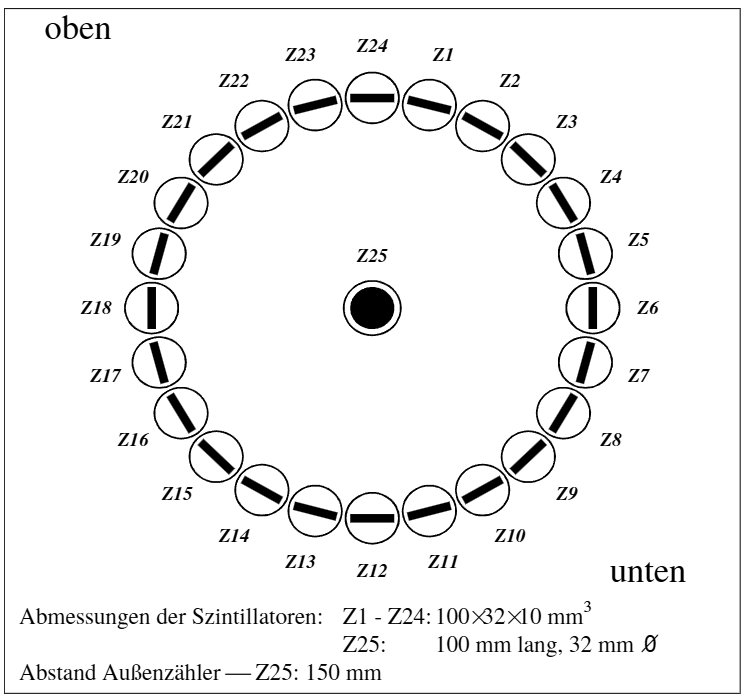
\includegraphics[width=0.48\textwidth]{figs/aufbau_winkel.png}
    \caption{Skizze der Versuchsanordnung für die Messung der Winkelverteilung der Höhenstrahlung \cite{praktikum}}
    \label{fig:winkel_aufbau}
\end{figure}

Die Ereignisse wurden mittels Drei-Koinzidenz-Darstellung erfasst. Dazu werden die analogen Ausgangssignale aller Szintillatoren zunächst über Vorverstärker an Differenzwandler geleitet, die sie in digitale Logikimpulse mit geringer Amplitude umwandeln. Die Differenz zwischen den Signalen der beiden äußeren Detektoren und denen des zentralen Detektors (Z25) bildet die Koinzidenzeinheit. (siehe Abbildung \ref{fig:winkel_elektronik})

\begin{figure}[H]
    \centering
    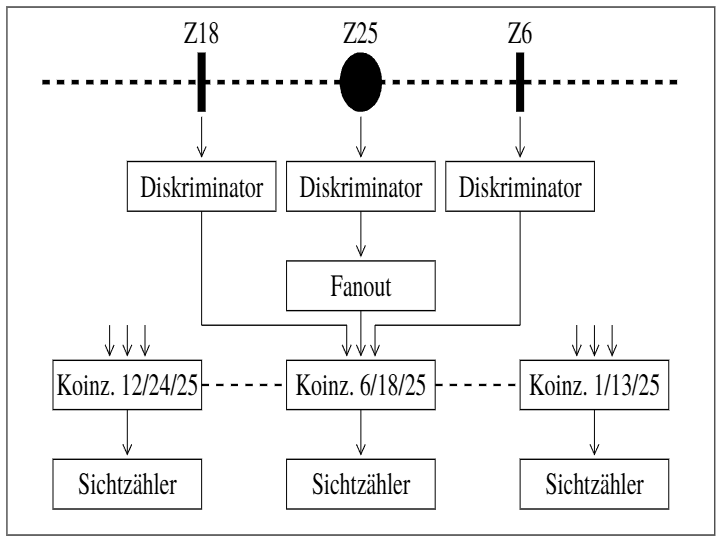
\includegraphics[width=0.48\textwidth]{figs/elektronik_winkel.png}
    \caption{Blockschaltbild der Elektronik zur Messung der Winkelverteilung \cite{praktikum}}
    \label{fig:winkel_elektronik}
\end{figure}

Dieses Verfahren liefert nur dann ein korrektes Ergebnis, wenn das Logiksignal innerhalb eines vorgegebenen Zeitintervalls gleichzeitig an allen drei Eingängen anliegt. Die Koinzidenzeinheit entspricht Myonen, die das Gerät in zufälliger Richtung passieren und denen ein bestimmter Azimutwinkel zugeordnet werden kann.

Durch die Untersuchung zweier verschiedener Detektorgruppen lässt sich die Flugbahn der Myonen in der oberen Hemisphäre berechnen. Das Produkt der Zählwerte über ein 15°-Intervall ergibt die Verteilung der Höhenstrahlung. 

\subsection{Teil 2: Messung der Lebensdauer der Muonen}
Im zweiten Teil des Experiments wird die Lebensdauer des Myons ermittelt. Hierfür wurde der in Abbildung \ref{fig:aufbau_myon} dargestellte Versuchsaufbau verwendet. Eine 5 cm dicke Bleiplatte schirmt den schmalen Photonenstrahl ab und lenkt ihn auf das Substrat.

\begin{figure}[H]
    \centering
    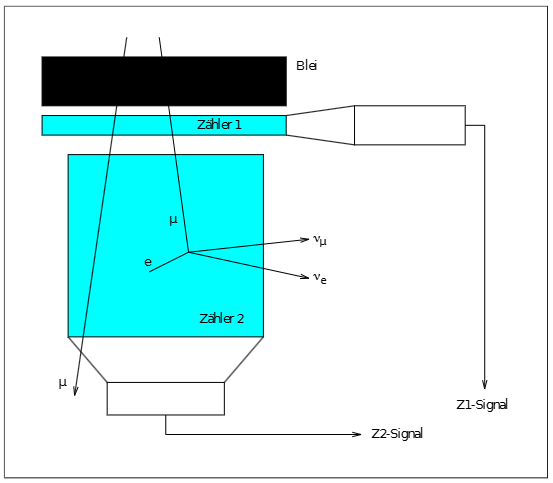
\includegraphics[width=0.48\textwidth]{figs/aufbau_myon.png}
    \caption{Schema des Aufbaus zur Messung der Myonlebensdauer \cite{praktikum}}
    \label{fig:aufbau_myon}
\end{figure}

Wenn ein einfallendes Photon auf zwei übereinanderliegende Detektoren trifft, emittiert es gleichzeitig in beiden ein elektrisches Signal. Dieses Signal dient als Startsignal für die Lebensdauermessungen. Der untere Szintillationsdetektor (Z2) ist massereich genug, um einige Myonen einzufangen und zu neutralisieren. Der bei der Kollision erzeugte elektrische Impuls erzeugt in Z2 ein zweites Signal, das als Stoppsignal aufgezeichnet wird.

Die Zeitdifferenz zwischen Start- und Stoppsignal wird manuell erfasst und durch eine von zehn $1\mu s$-Taktperioden dividiert. Die Zählrate des Detektors folgt dem erwarteten Trend, wodurch die Myonlebensdauer bestimmt werden kann.

Da das Gerät das Stoppsignal eines einfallenden Myons nicht von dem seines Zerfalls unterscheiden kann, wird für jeden Startimpuls ohne weitere Verarbeitung ein Stoppsignal erzeugt. Um dieses Problem zu beheben, wird das Startsignal mithilfe eines Verzögerungskabels um 100 ns gegenüber dem Stoppsignal verzögert. Dadurch werden die Stoppsignale der einfallenden Myonen zufällig. Diese Maßnahme bewirkt automatisch eine lineare Variation in der gemessenen Zeitverteilung, beeinflusst aber weder das exponentielle Verhalten noch die durch Anpassung ermittelten Lebensdauern.
